\documentclass[12pt,a4paper,fontset=none]{ctexart}

\usepackage[a4paper,margin=1.7cm]{geometry}
\usepackage{fontspec}
\usepackage{amsmath,amssymb}
\usepackage{array,booktabs,tabularx}
\usepackage{enumitem}
\usepackage{fancyhdr}
\usepackage{float}
\usepackage{graphicx}
\usepackage{hyperref}
\usepackage{listings}
\usepackage[most]{tcolorbox}
\usepackage{tikz}
\usepackage[table]{xcolor}

\usetikzlibrary{arrows.meta,positioning,shapes.geometric,shapes.multipart,fit,backgrounds,calc,trees,decorations.pathreplacing}

\hypersetup{colorlinks=true,linkcolor=black,urlcolor=blue}
\setmainfont{Times New Roman}
\setsansfont{Arial}
\setmonofont{Menlo}
\setCJKmainfont{Songti SC}
\setCJKsansfont{Heiti SC}
\setCJKmonofont{Songti SC}
\pagestyle{fancy}
\fancyhf{}
\fancyhead[L]{编译器构造实验 Lab3 — 实验一}
\fancyhead[R]{Oberon-0 语言定义}
\fancyfoot[C]{\thepage}
\setlength{\headheight}{15pt}
\setlist[itemize]{leftmargin=1.8em,itemsep=0.25em,topsep=0.35em}
\setlist[enumerate]{leftmargin=1.8em,itemsep=0.25em,topsep=0.35em}
\renewcommand{\arraystretch}{1.22}
\newcolumntype{P}[1]{>{\raggedright\arraybackslash}p{#1}}
\newcolumntype{Y}{>{\raggedright\arraybackslash}X}
\setlength{\emergencystretch}{2em}
\sloppy

\definecolor{accent}{HTML}{9A3412}
\definecolor{accenttwo}{HTML}{0F4C81}
\definecolor{accentthree}{HTML}{2F6B3D}
\definecolor{softa}{HTML}{F8EEE8}
\definecolor{softb}{HTML}{E8F0F7}
\definecolor{softc}{HTML}{EAF5ED}
\definecolor{linegray}{HTML}{D7CEC5}
\definecolor{codebg}{HTML}{F7F4EF}
\definecolor{boxbg}{HTML}{FCFAF7}
\definecolor{darktext}{HTML}{1F1B17}

\lstdefinestyle{labcode}{
  basicstyle=\ttfamily\small,
  backgroundcolor=\color{codebg},
  frame=single,rulecolor=\color{linegray},
  columns=fullflexible,keepspaces=true,
  showstringspaces=false,breaklines=true,
  keywordstyle=\color{accenttwo}\bfseries,
  commentstyle=\color{accentthree},
  stringstyle=\color{accent},
  aboveskip=0.5em,belowskip=0.5em
}

\lstdefinestyle{oberoncode}{
  basicstyle=\ttfamily\small,
  backgroundcolor=\color{codebg},
  frame=single,rulecolor=\color{linegray},
  columns=fullflexible,keepspaces=true,
  showstringspaces=false,breaklines=true,
  keywordstyle=\color{accenttwo}\bfseries,
  commentstyle=\color{accentthree}\itshape,
  stringstyle=\color{accent},
  emph={MODULE,PROCEDURE,BEGIN,END,CONST,TYPE,VAR,RECORD,ARRAY,OF,
        IF,THEN,ELSIF,ELSE,WHILE,DO,DIV,MOD,OR,INTEGER,BOOLEAN,TRUE,FALSE},
  emphstyle=\color{accenttwo}\bfseries,
  aboveskip=0.5em,belowskip=0.5em
}

\newtcolorbox{summaryBox}{enhanced,colback=softb,colframe=accenttwo,boxrule=0.8pt,
  arc=1.2mm,left=2.5mm,right=2.5mm,top=2mm,bottom=2mm,before upper=\raggedright}
\newtcolorbox{plainBox}{enhanced,colback=boxbg,colframe=linegray,boxrule=0.7pt,
  arc=1.2mm,left=2.3mm,right=2.3mm,top=1.8mm,bottom=1.8mm,before upper=\raggedright}
\newtcolorbox{keypointBox}{enhanced,colback=softc,colframe=accentthree,boxrule=0.8pt,
  arc=1.2mm,left=2.5mm,right=2.5mm,top=2mm,bottom=2mm,before upper=\raggedright}

\newcommand{\metric}[3]{
  \begin{minipage}[t]{0.19\linewidth}
    \begin{tcolorbox}[colback=boxbg,colframe=linegray,boxrule=0.7pt,arc=1mm,left=1.5mm,right=1.5mm,top=1.2mm,bottom=1.2mm]
      {\small\color{gray}#1}\par\vspace{1mm}
      {\large\bfseries\textcolor{#3}{#2}}
    \end{tcolorbox}
  \end{minipage}
}

% TikZ styles for diagrams
\tikzset{
  grammarnode/.style={draw,rounded corners=2mm,fill=softb,minimum width=2.2cm,minimum height=0.9cm,align=center,font=\small},
  tokennode/.style={draw,rounded corners=2mm,fill=softc,minimum width=2cm,minimum height=0.8cm,align=center,font=\small\ttfamily},
  errornode/.style={draw,rounded corners=2mm,fill=softa,minimum width=2.2cm,minimum height=0.8cm,align=center,font=\small},
  levelnode/.style={draw,rounded corners=1.5mm,fill=boxbg,minimum width=3.2cm,minimum height=0.85cm,align=center,font=\small\bfseries},
  arrow/.style={-{Latex[length=2mm]},thick,accenttwo},
  dasharrow/.style={-{Latex[length=2mm]},thick,dashed,accent},
  label/.style={font=\footnotesize\color{darktext}}
}

\title{{\Huge\bfseries 编译器构造实验 Lab3 实验一报告}\\[0.4em]{\Large 熟悉 Oberon-0 语言定义}}
\author{梁力航\quad 23336128}
\date{2026年5月20日}

\begin{document}

\begin{titlepage}
  \centering\vspace*{1.4cm}
  {\Large 中山大学计算机学院\par}\vspace{1.1cm}
  {\Huge\bfseries 编译器构造实验 Lab3 实验一报告\par}\vspace{0.45cm}
  {\LARGE 熟悉 Oberon-0 语言定义\par}\vspace{1cm}

  \begin{tcolorbox}[width=0.9\textwidth,colback=boxbg,colframe=linegray,boxrule=0.8pt,arc=1.5mm]
    本报告对应 ROSE 项目实验一：编写正确的 Oberon-0 源程序及变异程序，讨论语言特点和文法二义性。
  \end{tcolorbox}

  \vspace{0.9cm}
  \begin{tabular}{>{\bfseries}p{3.2cm}p{8.8cm}}
    课程 & 编译器构造实验（DCS292） \\
    实验名称 & Lab3 实验一：熟悉 Oberon-0 语言定义 \\
    姓名 & 梁力航 \\
    学号 & 23336128 \\
    日期 & 2026年5月20日 \\
    运行环境 & OpenJDK 11.0.24 / macOS / XeLaTeX
  \end{tabular}

  \vfill
  \metric{语法构造覆盖}{全部}{accent}\hfill
  \metric{正确程序}{1 个}{accenttwo}\hfill
  \metric{变异程序}{16 个}{accentthree}\hfill
  \metric{词法错误}{6 类}{accent}\hfill
  \metric{语法/语义错误}{10 类}{accentthree}
  \vfill
\end{titlepage}

\tableofcontents\newpage

% ===================================================================
\section{Oberon-0 语言概览}

Oberon-0 是 Niklaus Wirth 设计的 Oberon 语言的精简教学子集。它承袭了 Pascal 家族的块结构、强类型和结构化控制流，但刻意去除了复杂特性以保持语法简洁。

\begin{figure}[H]\centering
\begin{tikzpicture}[node distance=0.9cm and 1.5cm]
  % Language lineage
  \node[grammarnode,fill=accenttwo,text=white,font=\small\bfseries] (algol) {Algol 60\\(1960)};
  \node[grammarnode,right=of algol] (pascal) {Pascal\\(1970)};
  \node[grammarnode,right=of pascal] (modula) {Modula-2\\(1980)};
  \node[grammarnode,right=of modula,fill=accentthree,text=white,font=\small\bfseries] (oberon) {Oberon\\(1990)};
  \node[grammarnode,below=of oberon,fill=accent,text=white,font=\small\bfseries] (oberon0) {Oberon-0\\(本实验)};

  \draw[arrow] (algol) -- (pascal);
  \draw[arrow] (pascal) -- (modula);
  \draw[arrow] (modula) -- (oberon);
  \draw[arrow] (oberon) -- (oberon0);

  % Characteristics
  \node[font=\footnotesize,below=0.4cm of algol,text=darktext] {块结构、BNF定义};
  \node[font=\footnotesize,below=0.4cm of pascal,text=darktext] {强类型、结构化};
  \node[font=\footnotesize,below=0.4cm of modula,text=darktext] {模块化、信息隐藏};
  \node[font=\footnotesize,below=0.4cm of oberon,text=darktext] {精简、类型扩展};
  \node[font=\footnotesize,below=0.4cm of oberon0,text=darktext] {约50条EBNF规则};
\end{tikzpicture}
\caption{Oberon-0 的语言谱系——继承自四十年语言设计演进}
\label{fig:lineage}
\end{figure}

Oberon-0 的设计哲学是"足够简单以用于教学，又足够完整以体现高级语言的本质"：
\begin{itemize}
  \item 仅 INTEGER 和 BOOLEAN 两种基本类型——没有浮点、字符、字符串、指针
  \item 仅 IF/WHILE 两种控制结构——没有 FOR、REPEAT、CASE、GOTO
  \item 支持复合类型 ARRAY 和 RECORD——允许嵌套
  \item 支持 PROCEDURE 含值参数和 VAR 可变参数——过程抽象
  \item 模块作为唯一编译单元——程序组织
\end{itemize}

% ===================================================================
\section{Oberon-0 语言特点}

\subsection{保留字与关键字的区别}

Oberon-0 延续 Pascal 家族一个重要的设计传统：严格区分保留字（Reserved Word）和关键字（Keyword）。这在 C/Java 族语言中是不存在的概念。

\begin{table}[H]\centering
\begin{tabularx}{\textwidth}{>{\bfseries}P{2.5cm}Y>{\bfseries}P{2.5cm}Y}
\toprule
\multicolumn{2}{c}{\textbf{保留字（19 个）}} & \multicolumn{2}{c}{\textbf{关键字（7 个）}} \\
\midrule
模块结构 & MODULE, BEGIN, END & 预定义类型 & INTEGER, BOOLEAN \\
声明 & CONST, TYPE, VAR, PROCEDURE & 布尔值 & TRUE, FALSE \\
控制流 & IF, THEN, ELSIF, ELSE, WHILE, DO & 预定义过程 & READ, WRITE, WRITELN \\
类型构造 & ARRAY, OF, RECORD & & \\
运算符保留 & DIV, MOD, OR & & \\
\bottomrule
\end{tabularx}
\caption{保留字与关键字分类}
\end{table}

\begin{keypointBox}
\textbf{核心区别}：
\begin{itemize}
  \item \textbf{保留字}是语法结构的一部分，词法分析器将其识别为独立 token 类型。程序员\textbf{不能}将其声明为标识符。例如 \texttt{MODULE} 永远不能用作变量名
  \item \textbf{关键字}是预定义标识符，遵循标识符的作用域规则。程序员\textbf{可以}在内层作用域重新声明它们。例如可以在 PROCEDURE 内部声明 \texttt{VAR write: INTEGER;} 来遮蔽预定义过程 WRITE
  \item 这种区分使语言更容易扩展——新增预定义过程（如 Read）不改变语法本身
\end{itemize}
\end{keypointBox}

\subsection{表达式优先级层次}

Oberon-0 的表达式仅分 4 个优先级层，远少于 C/Java 的 15+ 层。这种简化是通过 BNF 的非终结符分层实现的：

\begin{figure}[H]\centering
\begin{tikzpicture}[node distance=0.7cm and 0cm]
  \node[levelnode,fill=accenttwo,text=white] (expr) {expression\\关系运算层 \texttt{= \# < <= > >=}};
  \node[levelnode,below=of expr,fill=accenttwo!80!white,text=white] (simple) {simple\_expression\\加减层 \texttt{+ - OR}};
  \node[levelnode,below=of simple,fill=accenttwo!60!white,text=white] (term) {term\\乘除层 \texttt{* DIV MOD \&}};
  \node[levelnode,below=of term,fill=accenttwo!40!white,text=white] (factor) {factor\\基本单元 + 取反 \texttt{\~{}}};

  \draw[arrow,white] (expr) -- (simple);
  \draw[arrow,white] (simple) -- (term);
  \draw[arrow,white] (term) -- (factor);

  % Right side: operators
  \node[right=4.5cm of expr,font=\small\ttfamily,text=accent] (op1) {a = b \quad a \# b \quad a < b};
  \node[right=4.5cm of simple,font=\small\ttfamily,text=accent] (op2) {a + b \quad a - b \quad a OR b};
  \node[right=4.5cm of term,font=\small\ttfamily,text=accent] (op3) {a * b \quad a DIV b \quad a MOD b \quad a \& b};
  \node[right=4.5cm of factor,font=\small\ttfamily,text=accent] (op4) {identifier \quad 123 \quad (expr) \quad \~{}flag};
\end{tikzpicture}
\caption{表达式优先级的分层设计——每层对应一个非终结符}
\label{fig:precedence}
\end{figure}

\begin{plainBox}
\textbf{关键差异}：与 C/Java 不同，Oberon-0 不支持关系运算符链（如 \texttt{a < b < c}），因为关系运算的结果是 BOOLEAN 类型，而 BOOLEAN 不能参与关系比较。这实际消除了 C 中 \texttt{0 < x < 10} 这类语义陷阱。
\end{plainBox}

\subsection{表达式语法对比：Oberon-0 vs Java/C/C++}

\begin{table}[H]\centering
\begin{tabularx}{\textwidth}{>{\bfseries}P{3cm}YY}
\toprule
特性 & Oberon-0 & Java / C / C++ \\
\midrule
运算符优先级层数 & 4 层 & 15+ 层 \\
逻辑与 & \texttt{\&}（无短路求值） & \texttt{\&\&}（短路求值） \\
逻辑或 & \texttt{OR}（无短路求值） & \texttt{||}（短路求值） \\
取反 & \texttt{\~{}} & \texttt{!} \\
不等号 & \texttt{\#} & \texttt{!=} \\
整除 & \texttt{DIV}（仅整数除法） & \texttt{/}（类型决定行为） \\
取模 & \texttt{MOD} & \texttt{\%} \\
关系运算符链 & 不支持 & C 支持，Java 不支持 \\
算术类型 & 仅 INTEGER & int/long/float/double 等 \\
布尔常量字面量 & 无（TRUE/FALSE是标识符） & true/false（保留字/字面量） \\
字符串类型 & 不支持 & 支持 \\
\bottomrule
\end{tabularx}
\caption{表达式语法差异详细对比}
\end{table}

% ===================================================================
\section{文法二义性分析}

\subsection{为什么 Oberon-0 文法无二义性}

Oberon-0 的 EBNF 文法\textbf{不存在二义性}。这不是偶然的——Wirth 在设计时有意避免了引起二义性的语法构造。以下从四个维度证明。

\subsection*{证据 1：表达式分层的优先级编码}

Oberon-0 没有像 yacc 那样用独立声明定义优先级，而是\textbf{通过非终结符的嵌套层次隐式编码了优先级和结合性}：

\begin{figure}[H]\centering
\begin{tikzpicture}[
  level 1/.style={sibling distance=5.5cm,level distance=1.3cm},
  level 2/.style={sibling distance=3cm,level distance=1.3cm},
  level 3/.style={sibling distance=1.5cm,level distance=1.3cm},
  every node/.style={grammarnode,font=\footnotesize\ttfamily}
]
\node {expression}
  child {node {simple\_expr}
    child {node {term}
      child {node {factor}}
    }
  }
  child {node[fill=softa,font=\footnotesize] {关系运算符\\= \# < <= > >=}}
  child {node[font=\footnotesize] (se2) {simple\_expr}
    child[missing]
    child[missing]
    child[missing]
  };

\draw[arrow,dashed] (se2) -- ++(0,-0.8);
\end{tikzpicture}
\caption{expression 规则的语法树——关系运算在最外层，不可能出现于更内层}
\label{fig:exprtree}
\end{figure}

因为 factor 只能包含 \texttt{( expression )}（带括号），所以 \texttt{a < b} 永远不可能出现在 term 或 factor 的上下文中——只有在 expression 层才会匹配关系运算符。这种分层本身就消除了所有中缀运算符的二义性问题。

\subsection*{证据 2：IF-END 消除 dangling-else}

经典 C/Java 的 dangling-else 问题：

\begin{figure}[H]\centering
\begin{tikzpicture}[node distance=0.6cm and 1.2cm]
  % C version
  \node[grammarnode,fill=softa,font=\small\bfseries] (ctitle) at (0,0) {C 语言：二义};
  \node[grammarnode,below=of ctitle,font=\footnotesize\ttfamily,minimum width=5cm,text width=4.8cm,align=left] (ccode) {
    if (a > 0)\\
    \quad if (b > 0) x = 1;\\
    \quad else x = 2;  // 属于哪个 if ?
  };

  % Oberon version
  \node[grammarnode,fill=softc,font=\small\bfseries] (otitle) at (7,0) {Oberon-0：无歧义};
  \node[grammarnode,below=of otitle,font=\footnotesize\ttfamily,minimum width=5cm,text width=4.8cm,align=left] (ocode) {
    IF a > 0 THEN\\
    \quad IF b > 0 THEN\\
    \quad\quad x := 1\\
    \quad END\\
    ELSE\\
    \quad x := 2\\
    END
  };

  % Highlight
  \draw[arrow,accent,line width=1.2pt] (ccode.east) -- (ocode.west) node[midway,above,font=\small\color{accent}] {消除歧义};
\end{tikzpicture}
\caption{dangling-else 消除对比}
\label{fig:dangling}
\end{figure}

因为每个 IF 都必须以 \texttt{END} 关键字显式关闭，所以 \texttt{ELSE} 属于哪个 \texttt{IF} 被明确界定——它属于最近一个尚未关闭的 IF。嵌套两个 IF 的 Oberon-0 代码中，\texttt{END} 明确关闭内层 IF 后，\texttt{ELSE} 自然归属外层 IF。

\subsection*{证据 3：选择符的后缀语法}

记录域访问 \texttt{.field} 和数组下标 \texttt{[index]} 都采用后缀形式，天然左结合。没有 C 中 \texttt{*p++} 这类前缀/后缀混合运算符导致的歧义。

\subsection*{证据 4：无空语句问题}

\begin{plainBox}
在 C 语言中，\texttt{if (x) ; y = 0;} 是合法但危险的——多余的分号创建了空语句，条件块为空。Oberon-0 中不存在此问题，因为：
\begin{enumerate}
  \item 语句之间用 \texttt{;} 分隔（而非终止），末尾不需要分号
  \item IF 语句必须包含至少一个 THEN 分支和 END 闭括号
\end{enumerate}
\end{plainBox}

\begin{summaryBox}
\textbf{二义性分析小结}：Oberon-0 通过三种机制消除二义性——(1) 非终结符分层编码优先级，(2) 闭括号 END 消除 dangling-else，(3) 后缀选择符和强制语句边界。这些设计决策体现了 Wirth "简洁即安全" 的理念。
\end{summaryBox}

% ===================================================================
\section{正确的 Oberon-0 源程序}

\subsection{程序功能说明}

\texttt{Sample.obr} 实现了一个简化的银行账户管理系统：

\begin{itemize}
  \item 使用 RECORD 定义账户类型（id + balance），ARRAY 存储账户列表
  \item 提供存款（Deposit）、取款（Withdraw）两个带 VAR 参数的过程
  \item 提供汇总统计（Summarize）、奖金检查（CheckBonus）、平均计算（ComputeAverage）、空账户检测（IsEmpty）等辅助过程
  \item 主程序初始化 100 个账户并依次调用各过程
\end{itemize}

该程序故意使用了 Oberon-0 的全部语法构造，不追求业务逻辑最优。

\subsection{完整源代码}

\begin{lstlisting}[style=oberoncode,caption={Sample.obr — 覆盖全部语法构造的正确 Oberon-0 程序}]
(* Sample.obr - A correct Oberon-0 source program.
   Covers ALL grammar constructs: MODULE, CONST, TYPE, VAR,
   PROCEDURE (value + VAR params), IF/THEN/ELSIF/ELSE, WHILE,
   arithmetic (+, -, *, DIV, MOD), comparisons (=, #, <, <=, >, >=),
   logical (&, OR, ~), array/record selectors (.field, [index]),
   predefined procedures (Read, Write, WriteLn) *)

MODULE Sample;
  CONST maxAccounts = 100; bonusRate = 5;
  TYPE
    AccountRec = RECORD
      id: INTEGER; balance: INTEGER
    END;
    AccountList = ARRAY maxAccounts OF AccountRec;
  VAR
    accounts: AccountList;
    totalBalance, count, i: INTEGER;
    hasBonus: BOOLEAN;

  PROCEDURE Max(a: INTEGER; b: INTEGER);
    VAR result: INTEGER;
  BEGIN
    IF a > b THEN result := a
    ELSE result := b
    END;
    Write(result); WriteLn
  END Max;

  PROCEDURE Deposit(VAR acc: AccountRec; amount: INTEGER);
  BEGIN
    acc.balance := acc.balance + amount;
    Write(acc.balance); WriteLn
  END Deposit;

  PROCEDURE Summarize;
    VAR k, temp: INTEGER;
  BEGIN
    totalBalance := 0; count := 0; k := 0;
    WHILE k < maxAccounts DO
      temp := accounts[k].balance;
      IF temp > 0 THEN
        totalBalance := totalBalance + temp;
        count := count + 1
      ELSIF temp = 0 THEN count := count + 1
      ELSE Write(0)
      END;
      k := k + 1
    END;
    Write(totalBalance); Write(count); WriteLn
  END Summarize;

  PROCEDURE CheckBonus(VAR ok: BOOLEAN; minBal: INTEGER);
    VAR j: INTEGER;
  BEGIN
    j := 0; ok := TRUE;
    WHILE (j < maxAccounts) & ok DO
      ok := accounts[j].balance >= minBal;
      j := j + 1
    END;
    ok := ok OR (j = 0);
    Write(j); WriteLn
  END CheckBonus;

  PROCEDURE ComputeAverage(VAR avg: INTEGER);
    VAR sum, cnt: INTEGER;
  BEGIN
    sum := 0; cnt := 0; i := 0;
    WHILE i < maxAccounts DO
      IF accounts[i].balance > 0 THEN
        sum := sum + accounts[i].balance;
        cnt := cnt + 1
      END;
      i := i + 1
    END;
    IF cnt > 0 THEN avg := sum DIV cnt
    ELSE avg := 0
    END;
    Write(avg); WriteLn
  END ComputeAverage;

  PROCEDURE IsEmpty(VAR empty: BOOLEAN);
    VAR m: INTEGER;
  BEGIN
    empty := TRUE; m := 0;
    WHILE (m < maxAccounts) & empty DO
      empty := accounts[m].balance = 0;
      m := m + 1
    END;
    empty := ~empty
  END IsEmpty;

BEGIN
  Read(i);  (* demonstrate READ *)
  i := 0;
  WHILE i < maxAccounts DO
    accounts[i].id := i + 1;
    accounts[i].balance := i * bonusRate;
    i := i + 1
  END;
  Max(10, 20);
  Deposit(accounts[0], 100);
  Withdraw(accounts[1], 10);
  Summarize;
  CheckBonus(hasBonus, 10);
  ComputeAverage(totalBalance);
  IsEmpty(hasBonus)
END Sample.
\end{lstlisting}

\subsection{语法构造覆盖矩阵}

\begin{table}[H]\centering
\scriptsize
\begin{tabularx}{\textwidth}{>{\bfseries}P{3.2cm}YP{2.5cm}}
\toprule
语法构造 & Sample.obr 中的使用 & 行号 \\
\midrule
MODULE + BEGIN..END 主体 & \texttt{MODULE Sample; ... END Sample.} & 16--147 \\
CONST 声明 & \texttt{maxAccounts = 100; bonusRate = 5} & 17--18 \\
TYPE RECORD & \texttt{AccountRec = RECORD id: INTEGER; balance: INTEGER END} & 20--23 \\
TYPE ARRAY & \texttt{AccountList = ARRAY maxAccounts OF AccountRec} & 24 \\
VAR (INTEGER + BOOLEAN) & \texttt{accounts, totalBalance, count, i: INTEGER; hasBonus: BOOLEAN} & 26--28 \\
PROCEDURE 值参 & \texttt{Max(a: INTEGER; b: INTEGER)} & 31 \\
PROCEDURE VAR 参数 & \texttt{Deposit(VAR acc: AccountRec; amount: INTEGER)} & 44 \\
PROCEDURE 无参 & \texttt{Summarize}, \texttt{ComputeAverage}, \texttt{IsEmpty} & 56,97,119 \\
IF/THEN/ELSE & \texttt{IF a > b THEN result := a ELSE result := b END} & 34--38 \\
IF/ELSIF/ELSE & \texttt{IF temp > 0 THEN ... ELSIF temp = 0 THEN ... ELSE ... END} & 65--71 \\
WHILE & \texttt{WHILE k < maxAccounts DO ... END} & 62--73 \\
算术 (+, -, *, DIV, MOD) & \texttt{sum DIV cnt}, \texttt{balance * bonusRate}, \texttt{k + 1} & 112,138,67 \\
比较 (=, \#, <, <=, >, >=) & \texttt{>=}, \texttt{<}, \texttt{=}, \texttt{>}, \texttt{<=} & 34,62,65,69,114 \\
逻辑 (\&, OR, \~{}) & \texttt{ok OR (j = 0)}, \texttt{(j < maxAccounts) \& ok}, \texttt{\~{}empty} & 94,89,128 \\
选择符 (.field, [index]) & \texttt{accounts[i].balance}, \texttt{accounts[k].balance} & 63,45 \\
READ & \texttt{Read(i)} & 132 \\
WRITE / WRITELN & \texttt{Write(avg); WriteLn} & 116 \\
\bottomrule
\end{tabularx}
\caption{完整语法构造覆盖矩阵}
\label{tab:coverage}
\end{table}

\begin{plainBox}
\textbf{覆盖完整性}：Sample.obr 使用了 Oberon-0 定义的全部语法构造——模块声明、三种声明（CONST/TYPE/VAR）、带值参和 VAR 参数的过程、IF/THEN/ELSIF/ELSE 和 WHILE 控制结构、全部运算符层级、记录和数组选择符、三个预定义过程。
\end{plainBox}

% ===================================================================
\section{变异程序}

\subsection{变异测试方法}

变异测试（Mutation Testing）的思路是：对正确程序做出\textbf{最小改动}，植入\textbf{单一错误}，形成变异程序（Mutant）。如果测试工具能检测到这个错误，说明测试有效；如果检测不到，说明测试覆盖有空隙。

\begin{figure}[H]\centering
\begin{tikzpicture}[node distance=1cm and 1.8cm]
  \node[grammarnode,fill=softc,font=\small\bfseries] (correct) {正确程序\\Sample.obr};
  \node[grammarnode,right=of correct,font=\small] (m1) {变异 1\\@ 非法符号};
  \node[grammarnode,right=of m1,font=\small] (m2) {变异 2\\无空白整数};
  \node[font=\small,right=of m2] (dots) {$\cdots$};
  \node[grammarnode,right=of dots,font=\small] (m16) {变异 16\\名不匹配};

  \draw[arrow] (correct) -- (m1);
  \draw[arrow] (correct) -- (m2);
  \draw[arrow] (correct) -- (dots);
  \draw[arrow] (correct) -- (m16);
\end{tikzpicture}
\caption{变异测试方法：从正确程序派生出多个单点错误变体}
\label{fig:mutation}
\end{figure}

\subsection{变异程序示例代码}

三类错误的代表性变异程序：

\begin{lstlisting}[style=oberoncode,caption={词法错误：非法符号（Sample.001）}]
(* ERROR: IllegalSymbolException - @ symbol is not valid *)
MODULE Sample;
  VAR x: INTEGER;
BEGIN
  x := 5 @ 3       (* ← @ 不是 Oberon-0 的合法字符 *)
END Sample.
\end{lstlisting}

\begin{lstlisting}[style=oberoncode,caption={词法错误：八进制非法数字（Sample.005）}]
(* ERROR: IllegalOctalException - 8 not allowed in octal *)
MODULE Sample; VAR x: INTEGER;
BEGIN
  x := 018          (* ← 0 开头视为八进制，但含数字 8 *)
END Sample.
\end{lstlisting}

\begin{lstlisting}[style=oberoncode,caption={语法错误：缺少操作数（Sample.010）}]
(* ERROR: MissingOperandException *)
MODULE Sample; VAR x: INTEGER;
BEGIN
  x := 5 + ;        (* ← 运算符 + 后面缺少操作数 *)
  Write(x)
END Sample.
\end{lstlisting}

\begin{lstlisting}[style=oberoncode,caption={语义错误：类型不兼容（Sample.011）}]
(* ERROR: TypeMismatchedException - BOOLEAN in arithmetic *)
MODULE Sample;
  VAR x: INTEGER; flag: BOOLEAN;
BEGIN
  flag := TRUE;
  x := flag + 10    (* ← BOOLEAN 值不能参与算术运算 *)
END Sample.
\end{lstlisting}

\begin{lstlisting}[style=oberoncode,caption={语义错误：模块名不匹配（Sample.016）}]
(* ERROR: SemanticException - module name mismatch *)
MODULE Sample; VAR x: INTEGER;
BEGIN
  x := 100
END WrongName.      (* ← END 后的名字与 MODULE 声明不一致 *)
\end{lstlisting}

\subsection{完整变异程序清单}

\begin{table}[H]\centering
\tiny
\setlength{\tabcolsep}{2.5pt}
\begin{tabularx}{\textwidth}{>{\bfseries}P{1.2cm}>{\raggedright\arraybackslash}P{4.5cm}>{\raggedright\arraybackslash}P{3.5cm}>{\raggedright\arraybackslash}X}
\toprule
编号 & 错误特征 & 异常类型 & 错误阶段 \\
\midrule
\multicolumn{4}{c}{\textbf{词法错误（6 个）}} \\
Sample.001 & \texttt{5\char64 3}（非法字符） & IllegalSymbolException & 词法分析 \\
Sample.002 & \texttt{25id}（整数无空白接标识符） & IllegalIntegerException & 词法分析 \\
Sample.003 & 标识符长度 > 24 字符 & IllegalIdentifierLengthException & 词法分析 \\
Sample.004 & \texttt{(* unclosed}（注释未闭合） & MismatchedCommentException & 词法分析 \\
Sample.005 & \texttt{018}（八进制含数字 8） & IllegalOctalException & 词法分析 \\
Sample.006 & 整数 > 12 位 & IllegalIntegerRangeException & 词法分析 \\
\midrule
\multicolumn{4}{c}{\textbf{语法错误（7 个）}} \\
Sample.007 & \texttt{2 * 3 + 5)}（多余右括号） & MissingLeftParenthesisException & 语法分析 \\
Sample.008 & \texttt{(2 + 3 * 5}（缺少右括号） & MissingRightParenthesisException & 语法分析 \\
Sample.009 & \texttt{x 10}（两操作数间无运算符） & MissingOperatorException & 语法分析 \\
Sample.010 & \texttt{5 + ;}（运算符后缺操作数） & MissingOperandException & 语法分析 \\
Sample.014 & \texttt{IF ... 缺 THEN} & SyntacticException & 语法分析 \\
Sample.015 & \texttt{WHILE ... 缺 END} & SyntacticException & 语法分析 \\
Sample.016 & 模块 END 名字不匹配 & SemanticException & 语义分析 \\
\midrule
\multicolumn{4}{c}{\textbf{语义错误（3 个）}} \\
Sample.011 & \texttt{flag + 10}（BOOL + INTEGER） & TypeMismatchedException & 语义分析 \\
Sample.012 & \texttt{x \& TRUE}（INTEGER \& BOOL） & TypeMismatchedException & 语义分析 \\
Sample.013 & \texttt{Add(5)}（参数个数错误） & ParameterMismatchedException & 语义分析 \\
\bottomrule
\end{tabularx}
\caption{16 个变异程序完整清单——覆盖 3 个错误阶段、12 种异常类型}
\label{tab:mutants}
\end{table}

\subsection{异常类层次结构}

\begin{figure}[H]\centering
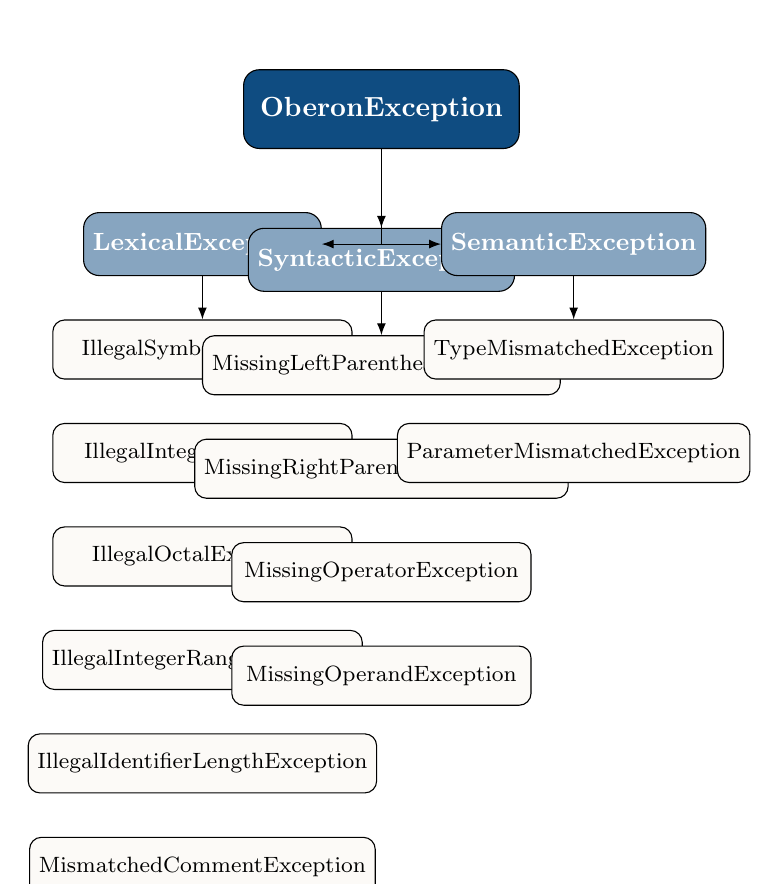
\begin{tikzpicture}[
  node distance=0.55cm and 0.3cm,
  root/.style={draw,rounded corners=2mm,fill=accenttwo,text=white,minimum width=3.5cm,minimum height=1cm,align=center,font=\bfseries},
  cat/.style={draw,rounded corners=2mm,fill=accenttwo!50!white,text=white,minimum width=3cm,minimum height=0.8cm,align=center,font=\small\bfseries},
  leaf/.style={draw,rounded corners=1.5mm,fill=boxbg,minimum width=3.8cm,minimum height=0.75cm,align=center,font=\footnotesize},
  line/.style={-{Latex[length=1.5mm]},thin}
]
  \node[root] (root) {OberonException};

  \node[cat,below left=0.8cm and -1cm of root] (lex) {LexicalException};
  \node[cat,below=1cm of root] (syn) {SyntacticException};
  \node[cat,below right=0.8cm and -1cm of root] (sem) {SemanticException};

  \draw[line] (root.south) |- (lex);
  \draw[line] (root) -- (syn);
  \draw[line] (root.south) |- (sem);

  % Lexical children
  \node[leaf,below=of lex] (l1) {IllegalSymbolException};
  \node[leaf,below=of l1] (l2) {IllegalIntegerException};
  \node[leaf,below=of l2] (l3) {IllegalOctalException};
  \node[leaf,below=of l3] (l4) {IllegalIntegerRangeException};
  \node[leaf,below=of l4] (l5) {IllegalIdentifierLengthException};
  \node[leaf,below=of l5] (l6) {MismatchedCommentException};
  \draw[line] (lex) -- (l1);

  % Syntactic children
  \node[leaf,below=of syn] (s1) {MissingLeftParenthesisException};
  \node[leaf,below=of s1] (s2) {MissingRightParenthesisException};
  \node[leaf,below=of s2] (s3) {MissingOperatorException};
  \node[leaf,below=of s3] (s4) {MissingOperandException};
  \draw[line] (syn) -- (s1);

  % Semantic children
  \node[leaf,below=of sem] (e1) {TypeMismatchedException};
  \node[leaf,below=of e1] (e2) {ParameterMismatchedException};
  \draw[line] (sem) -- (e1);
\end{tikzpicture}
\caption{异常类继承层次——3 个中间分类 + 12 个具体异常}
\label{fig:exceptions}
\end{figure}

% ===================================================================
\section{实验心得}

\begin{enumerate}
  \item \textbf{Oberon-0 的"小"体现了语言设计的"精"}。仅约 50 条 EBNF 规则就覆盖了模块化、结构化控制、过程抽象、复合类型等核心概念。相比之下，Java 语言规范超过 600 页。这种精简是经过深思熟虑的取舍——Wirth 去掉了所有可以省略而不影响表达能力的东西
  \item \textbf{文法设计直接影响实现复杂度}。非终结符分层隐式编码优先级的方式，使语法分析器不需要外部的优先级表或结合性声明，这比 yacc 风格的优先级指令更优雅——设计层面的清晰消除了实现层面的 hack
  \item \textbf{保留字与关键字的区分在实际实现中影响显著}。它决定了词法分析器中哪些标识符需要硬编码查找、哪些可以在符号表中动态管理。C/Java 把类型名也当作保留字，导致语言扩展（新增关键字）几乎不可能向后兼容；Oberon 的做法在这方面更灵活
  \item \textbf{变异测试方法很有实用价值}。在进入正式编码前先设计测试用例（特别是含有错误的变异程序），迫使先想清楚错误应该在哪个阶段检测、抛出什么异常。这实际上就是 TDD 思想在编译器测试中的具象化
\end{enumerate}

\begin{summaryBox}
实验一完成：1 个覆盖全部 15 类语法构造的正确 Oberon-0 源程序 Sample.obr；16 个变异程序覆盖 6 种词法错误、7 种语法错误、3 种语义错误（对应 12 个具体异常类）；Oberon-0 语言特点讨论（保留字/关键字区分 + 表达式对比）和四维文法二义性分析（分层优先级、IF-END、后缀选择符、无空语句）。
\end{summaryBox}

\end{document}
